\chapter{Seguridad} \label{sec:security}
	La palabra seguridad es empleada en multitud de situaciones dentro del mundo de las tecnologías de la información, normalmente con significados dispares. No obstante, generalizando lo suficiente, viene a referirse a la protección que se debe proporcionar a determinados recursos, por su valor y/o sensibilidad, frente a posibles usos malintencionados.
	
	Esta sección está dedicada a las cuestiones de seguridad, en sentido amplio, relacionadas con \href{https://firstmarket.tech}{FirstMarket}.
	\section{HTTPS} \label{sec:https}
	Como se ha comentado, una de los principales retos que afronta el comercio electrónico es la generación de confianza. Los usuarios demandan seguridad a la hora de realizar sus compras por la red. En este sentido, el desarrollo de protocolos seguros de comunicación ha jugado un papel protagonista en el rápido incremento que el comercio \emph{online} ha vivido en las últimas décadas.
	
	HTTPS, la extensión segura de HTTP, es el protocolo de comunicación segura por excelencia en la actualidad. Los datos enviados con HTTPS son protegidos mediante el protocolo Transport Layer Security (TLS), el cual brinda tres tipos de protección:
	
		\begin{itemize}
			\item[-] Privacidad. Los datos son encriptados antes de moverse por la red, de forma que nadie ajeno a la conversación pueda comprender su semántica.
			\item[-] Integridad. De una manera similar a como Git detecta los cambios en los documentos que gestiona, TLS calcula determinados parámetros criptográficos que hacen extremadamente difícil que los datos sean alterados en su camino por la red, ya sea accidental o intencionadamente, sin que el protocolo lo detecte.
			\item[-] Autenticidad. Aún teniendo garantizado que nadie podrá entender los datos enviados, y que nadie los podrá alterar sin notarse, persiste la duda de si se está comunicando con el interlocutor pretendido. Esto es, cuando alguien accede a www.firstmarket.tech debe tener la certeza de que efectivamente está intercambiando información con FirstMarket (hipotética persona jurídica). Para esta labor TLS hace uso de los certificados digitales, que un tercer agente \emph{de confianza} emite garantizando que la web de FirstMarket es www.firstmarket.tech. Este agente es el conocido en la industria como \emph{Certificate Authority} (CA). Pero, ¿quién establece la autoridad de este CA, es decir, quién asegura que es \emph{de confianza}? Otro CA, de mayor autoridad, y así sucesivamente. Esto crea una cadena de confianza, finita, englobada dentro de la \emph{Public Key Infrastructure} (PKI), la tecnología fundamental de Internet para construir la confianza acerca de la autenticidad de los agentes en la red.
		\end{itemize}
	
	La aplicación web desarrollada puede usar HTTPS, ya que por defecto este es el protocolo que Heroku proporciona para la comunicación de sus aplicaciones ejecutadas con \emph{dynos} de pago (como es el caso). En concreto, por defecto y sin coste añadido, Heroku gestiona los certificados digitales de las aplicaciones automáticamente con su servicio \href{https://devcenter.heroku.com/articles/automated-certificate-management}{\emph{Automated Certificate Management}} (ACM). Por su parte, ACM utiliza \href{https://letsencrypt.org/}{\emph{Let’s Encrypt}}, un CA abierto, gratuito y automatizado que ofrece para el bien común el \href{https://www.abetterinternet.org/}{\emph{Internet Security Research Group}}.
	
	Para finalizar, resaltar que \href{https://firstmarket.tech}{www.firstmarket.tech} impone el uso de HTTPS, es decir, los intentos de comunicarse con la aplicación web por medio de HTTP son redirigidos al uso de la versión segura. Esto se ha implementado con Spring Security, como se muestra entre las líneas 27 y 31 del listado \ref{list:springsec_config}.
	
	\section{Spring Security} \label{sec:springsec}
	Un enfoque comúnmente empleado, en el ámbito de la seguridad de la información, se basa en considerar los sistemas complejos como un conjunto de capas de abstracción, aplicándose los mecanismos de seguridad apropiados para cada una de ellas.
	
	Si se piensa en la aplicación de comercio electrónico que se ha desarrollado, esta puede modelarse en esencia como un proceso que se ejecuta en el contexto de un sistema operativo, en el seno a su vez de una máquina, la cual se comunica con otras haciendo uso de la infraestructura de Internet. Este modelo simple ya es capaz de hacer contraste entre la aplicación, el sistema operativo, la máquina y la red. Cada una de estas capas implementa sus propias medidas destinadas a proteger la información que maneja.
	
	A nivel de aplicación, los conceptos de autenticación y autorización (o acceso) son nucleares en su ámbito de seguridad. Autenticación hace referencia a la capacidad de la aplicación para identificar al usuario. Es decir, desde el punto de vista de la aplicación, responde a la pregunta ¿quién me está usando? Autorización, por su parte, refleja la capacidad de la aplicación de permitir, o denegar, el acceso a un recurso o funcionalidad de la aplicación a un determinado usuario. Como puede notarse, para que la aplicación pueda \emph{autorizar} a un usuario, debe primero \emph{autenticar} a dicho usuario.
	
	Spring Security es la piedra angular de la seguridad a nivel de aplicación del portal de comercio electrónico desarrollado, integrando las funcionalidades de autenticación y autorización encima de las características propias de Spring Framework. Además, como se verá, también ofrece mecanismos de protección frente a multitud de vulnerabilidades comunes a nivel de aplicación.
	
	\subsection{FilterChain}
	Como se comenta en la sección \ref{sec:spring}, las aplicaciones web con Spring basadas en el stack servlet, como es el caso, siguen el patrón \emph{front controller}, en el que el servlet \href{https://docs.spring.io/spring/docs/current/spring-framework-reference/web.html#mvc-servlet}{\emph{DispatcherServlet}} ejerce de punto de entrada y distribuidor de las peticiones HTTP hacia los \emph{@Controller}/\emph{@RestController} adecuados.
	
	El \emph{DispatcherServlet} no integra lógica de autenticación/autorización, por lo que, en ausencia de alternativas, esta debería ser implementada en las clases \emph{@Controller}/\emph{@RestController} en las que delega las peticiones HTTP. Esto, por supuesto, destrozaría el principio de separación de responsabilidades. 
	
	Afortunadamente, sí que existe alternativa, los Java \href{https://www.oracle.com/java/technologies/filters.html}{Filters}. Estos componentes interceptan el tráfico entrante y/o saliente de los servlets, permitiendo inyectar la lógica que se desee. Así, la autenticación/autorización puede ser implementada en estos \emph{filters}, de forma que las labores de seguridad sean llevadas a cabo antes de que las peticiones HTTP alcancen el \emph{DispatcherServlet}.
	
	Además, los \emph{filters} poseen la capacidad de concatenarse entre sí, creando un \emph{filter chain} o cadena de filtros, como se muestra en la figura \ref{fig:filterchain}, tomada de la documentación oficial de Spring Security. Esto permite, otra vez, separar responsabilidades, e insertar en cada filtro la lógica de una funcionalidad concreta.
	
	\begin{figure}[hbt!]
		\centering
		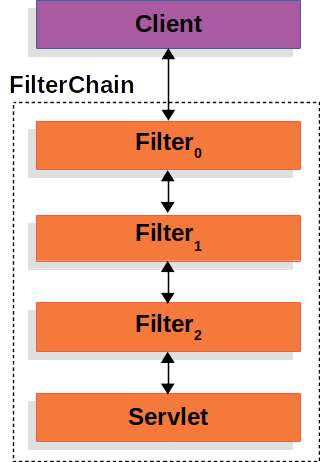
\includegraphics[width=0.4\textwidth,keepaspectratio]{filterchain}
		\caption{Encadenamiento de filtros}
		\label{fig:filterchain}
	\end{figure}
	
	Por ejemplo, una petición HTTP podría primero alcanzar un filtro destinado a recabar las credenciales de autenticación del usuario (por ejemplo un formulario de \emph{login}). Después, con dichas credenciales, atravesar el filtro que las comprueba, y autenticar así o no al usuario. Seguidamente podría estar el filtro que decide si el usuario recién autenticado posee el permiso necesario para acceder al recurso o funcionalidad pedida. Por último, en caso necesario, la petición HTTP llegaría al \emph{DispatcherServlet}.
	
	En el listado \ref{list:filter_chain} se aprecia el mensaje de registro emitido durante el arranque de la aplicación en el que se detalla la cadena de filtros que Spring Security proporciona. Pues bien, en esencia, \textbf{Spring Security \emph{es} esta concatenación de filtros} antes del \emph{DispatcherServlet}. 
	\\
	
	\begin{lstlisting}[caption=Cadena de filtros creada por Spring Security, label=list:filter_chain]
	2020-07-18 17:20:19.718  DefaultSecurityFilterChain: 
	Creating filter chain: any request, 
	[
	ChannelProcessingFilter, 
	WebAsyncManagerIntegrationFilter, 
	SecurityContextPersistenceFilter, 
	HeaderWriterFilter, 
	CsrfFilter, 
	LogoutFilter, 
	UsernamePasswordAuthenticationFilter, 
	RequestCacheAwareFilter, 
	SecurityContextHolderAwareRequestFilter, 
	AnonymousAuthenticationFilter, 
	SessionManagementFilter, 
	ExceptionTranslationFilter, 
	FilterSecurityInterceptor
	]
	\end{lstlisting}
	
	\subsection{Configuración}
	En estos filtros Spring Security implementa la autenticación/autorización y la protección frente a determinados tipos de ataques. Lo que resta es configurarlos para satisfacer las necesidades propias de cada aplicación. Esta configuración se lleva a cabo extendiendo la clase de Spring Security \emph{WebSecurityConfigurerAdapter} y sobreescribiendo su método \emph{configure(HttpSecurity)} (expuesto en el listado \ref{list:springsec_config}), tarea que en la aplicación web desarrollada realiza la clase \emph{SecurityConfig}.
	\\
	
	\begin{lstlisting}[caption=Configuración de Spring Security en FirstMarket, label=list:springsec_config]
	@Override
	protected void configure(HttpSecurity httpSecurity) throws Exception {
		httpSecurity
			// authenticate through login form
			.formLogin()
			.loginPage("/login")
			.failureHandler(customAuthenticationFailureHandler())
			
			// set logout page
			.and()
			.logout()
			.logoutSuccessUrl("/home")
			
			// authorization
			.and()
			.authorizeRequests()
			// protect role_admin resources
			.antMatchers("/admin/**")
			.access("hasRole('ROLE_ADMIN')")
			// protect role_user resources
			.antMatchers("/user/**")
			.access("hasRole('ROLE_USER')")
			// publicly open
			.antMatchers("/", "/home", "/login", "/newUser")
			.access("permitAll")
			
			// force HTTPS always
			.and()
			.requiresChannel()
			.antMatchers("/**")
			.requiresSecure()
			
			// enable csrf protection
			.and()
			.csrf()
			.ignoringAntMatchers("/listener") // open for stripe
			
			// always create new session
			.and()
			.sessionManagement()
			.sessionCreationPolicy(SessionCreationPolicy.ALWAYS)
			
			.and()
			.headers(headers -> headers
				// HTTP Strict Transport Security
				.httpStrictTransportSecurity(hsts -> hsts
					.includeSubDomains(true)
					.preload(true)
					.maxAgeInSeconds(31536000)
				)
				// Content Security Policy
				.contentSecurityPolicy(csp -> csp
					.policyDirectives("default-src 'none'" +
						"; " +
						"script-src 'self' " +
						"https://js.stripe.com " +
						"https://*.fontawesome.com " +
						"https://maxcdn.bootstrapcdn.com " +
						"https://cdnjs.cloudflare.com " +
						"https://ajax.googleapis.com" +
						"; " +
						"style-src 'self' " +
						"https://cdn.jsdelivr.net " +
						"https://maxcdn.bootstrapcdn.com " +
						"https://fonts.googleapis.com " +
						"https://*.fontawesome.com" +
						"; " +
						"font-src 'self' " +
						"https://fonts.gstatic.com " +
						"https://*.fontawesome.com" +
						"; " +
						"img-src 'self' data:" +
						"; " +
						"frame-src 'self' " +
						"https://js.stripe.com" +
						"; " +
						"connect-src 'self' " +
						"https://api.stripe.com"
					)
				)
				// Referrer Policy
				.referrerPolicy(referrer -> referrer
					.policy(ReferrerPolicyHeaderWriter.ReferrerPolicy.STRICT_ORIGIN)
				)
			)
		;
	}
	\end{lstlisting}
	
	\subsection{Autenticación}
	Spring Security ofrece toda una gama de métodos de autenticación. El usado en FirstMarket, configurado entre las líneas 5 y 7 del listado \ref{list:springsec_config}, ha sido a través de un formulario, contenido en la vista \emph{login.html}, en el que el usuario introduce su dirección de correo electrónico y su contraseña. En caso de un fallo de autenticación, la clase \emph{customAuthenticationFailureHandler} toma el control, determina la causa del fallo y presenta el mensaje adecuado al usuario.
	
	Es importante resaltar que, con el fin de garantizar la seguridad de la información de los usuarios, la aplicación web desarrollada almacena las constraseñas en la base de datos encriptadas.  En concreto, se usa el agoritmo \href{https://en.wikipedia.org/wiki/Bcrypt}{Bcrypt}. De esta forma, para saber si la contraseña es correcta, la aplicación web encripta la contraseña enviada en el formulario y la compara con la que tiene almacenada.
	
	Además, Spring Security permite especificar la lógica tras un \emph{logout}, que en el caso de la presente aplicación es simplemente una redirección a la páquina de inicio, como se muestra en las líneas 12 y 13 del listado \ref{list:springsec_config}.
	
	\paragraph{Autenticación por Fuerza Bruta}
	Como ya se ha comentado, el ecosistema Spring destaca por su extensibilidad. Allá donde se requieran funcionalidades especiales, el framework permite alcanzarlas. En este sentido, aunque Spring Security no implementa ningún mecanismo para prevenir la autenticación por fuerza bruta, sí ofrece facilidades para incorporarlo.
	
	Cada vez que un usuario trata de autenticarse, en función del éxito o del motivo del fracaso, Spring Security emite el correspondiente evento. Si la autenticación tuvo éxito se emite el evento \emph{AuthenticationSuccessEvent}, mientras que si fracasa por ser la información proporcionada incorrecta se emite \emph{AuthenticationFailureBadCredentialsEvent}. Otro motivos de fracaso (por ejemplo estar la cuenta de usuario bloqueada por el administrador) emiten diferentes eventos.
	
	Escuchando estos eventos, la aplicación web desarrollada implementa, con las clases contenidas en el paquete \emph{firstmarket.security},  una protección frente a intentos de autenticación por fuerza bruta. Esto es, se impide la posibilidad de probar sistemáticamente un número muy grande de contraseñas para descubrir cuál es la correcta.
	
	Para ello, la clase \emph{LockManager} mantiene un registro caché (usando la clase \emph{LoadingCache} de la librería \href{https://guava.dev/}{Guava}) con el que llevar el conteo de los intentos fallidos de autenticación, debido a credenciales incorrectas, dentro de una ventana temporal.
	
	Así, dentro de un tiempo determinado se restringe el número de intentos con credenciales fallidas, de forma que, si se supera el límite, la cuenta de usuario queda bloqueda temporalmente (por un tiempo igual a la ventana temporal). Por contra, si dentro de dicho intervalo, y sin haber superado el límite de intentos, se proporcionara las credenciales correctas, el registro se limpia. Además, cada entrada en la caché se limpia automáticamente tras superarse un tiempo igual a la ventana disponible sin que se haya producido un bloqueo.
	
	Tanto el número de intentos permitidos (\emph{num-of-attempts}) como la ventana temporal (\emph{locking-minutes}) son externalizados en el fichero de propieades de la aplicación, \emph{application.yml}. En el listado \ref{list:lock_params} se muestra su configuación en producción.
	\\
	
	\begin{lstlisting}[caption=Parámetros para configurar la prevención de autenticación por fuerza bruta,label=list:lock_params]
	fm:
		security:
			lock:
				num-of-attempts: 5
				locking-minutes: 60
	\end{lstlisting}
	

	\subsection{Autorización}
	Como se puede apreciar en el listado \ref{list:springsec_config}, líneas de la 15 a la 26, FirstMarket implementa tres tipos de recursos: 
	
	\begin{itemize}
		\item[-] Los que sólo pueden ser accedidos por los usuarios con rol \emph{ROLE\_ADMIN}, ubicados en \emph{\nolinkurl{~/admin/**}}.
		\item[-] Los que sólo pueden ser accedidos por los usuarios con rol \emph{ROLE\_USER}, ubicados en \emph{\nolinkurl{~/user/**}}.
		\item[-] El resto, que puede ser accedido por cualquiera.
	\end{itemize}

	Notar que los dos primeros tipos requieren necesariamente autenticación previa.
	
	\subsection{Cross-Site Request Forgery}
	\href{https://en.wikipedia.org/wiki/Cross-site_request_forgery}{\emph{Cross-Site Request Forgery}} representa un tipo de ataque que toma ventaja de la confianza que un determinado sitio web tiene en un cliente, por ejemplo porque previamente se ha autenticado. Así, el cliente envía (sin saberlo) una petición (maliciosa) al sitio web y este la acepta dada la confianza que deposita en el primero. Es el caso inverso a los ataques \href{https://owasp.org/www-community/attacks/xss/}{\emph{Cross-Site Scripting}}, donde se saca partido de la confianza que el cliente tiene en el sitio web, ejecutando el código (malicioso) que este le envía (sin saberlo).
	
	Imagínese que un usuario se encuentra, autenticado, en la aplicación web de su banco, en la vista que le permite transferir fondos de su cuenta a otra. Esta vista, por ejemplo, mostraría un formulario como el mostrado en el listado \ref{list:csrf_form}. Al completarlo y presionar \emph{Transfer} se enviaría al servidor del banco la petición HTTP mostrada en el listado \ref{list:csrf_http}.
	\\
	
	\begin{lstlisting}[caption=Formulario inseguro para la transferencia de fondos,label=list:csrf_form]
	<form method="post" action="/transfer">
		<input type="text" name="amount"/>
		<input type="text" name="account"/>
		<input type="submit" value="Transfer"/>
	</form>
	\end{lstlisting}
	
	\begin{lstlisting}[caption=Petición HTTP insegura para la transferencia de fondos,label=list:csrf_http]
	POST /transfer HTTP/1.1
	Host: bank.example.com
	Cookie: JSESSIONID=randomid
	Content-Type: application/x-www-form-urlencoded
	
	amount=100.00&account=9876
	\end{lstlisting}
	
	Hasta aquí todo normal, pero imagínese que, antes de realizar \emph{logout} en la aplicación del banco, se visita otro sitio web, el cual sirve al cliente el formulario mostrado en el listado \ref{list:csrf_form_evil}. Si en esta situación el usuario presiona \emph{Win Money!} se enviará al servidor una petición HTTP exactamente igual que la mostrada en el listado \ref{list:csrf_http}, salvo el número de cuenta a donde se envía el dinero. Es decir, el usuario habrá sido estafado.
	\\
	
	\begin{lstlisting}[caption=Formulario para la transferencia ilegítima de fondos,label=list:csrf_form_evil]
	<form method="post" action="https://bank.example.com/transfer">
		<input type="hidden" name="amount" value="100.00"/>
		<input type="hidden" name="account" value="evilAccountNum"/>
		<input type="submit" value="Win Money!"/>
	</form>
	\end{lstlisting}
	
	El banco no tiene posibilidad de distinguir si alguna de las dos peticiones es ilegítima, ya que en ambas cree que las está haciendo el usuario autorizado para ello. ¿Por qué? porque el medio que utiliza para identificar al usuario, la \emph{cookie} de la línea 3 del listado \ref{list:csrf_http}, es exactamente igual en ambas peticiones, ya que el navegador por defecto adjunta las cookies en todas las peticiones.
	
	La manera más extendida de solucionar este problema, que Spring Security implementa por defecto, es adjuntar una pieza de información extra (\emph{token}) que sólo conozca el usuario legítimo. Obviamente, este \emph{token} no puede ser colocado en una \emph{cookie}, porque se estaría en la misma situación vulnerable anteriormente descrita. En este sentido, existen diversas alternativas de lugares donde colocar el \emph{token}, siendo en un campo oculto (llamado \emph{\_csrf}) la utilizada por defecto en Spring Security. Así, el formulario que el banco enviaría ahora al usuario sería como el mostrado en el listado \ref{list:csrf_form_token}, mientras que la petición HTTP sería la mostrada en el listado \ref{list:csrf_http_token}.
	\\
	
	\begin{lstlisting}[caption=Formulario seguro para la transferencia de fondos,label=list:csrf_form_token]
	<form method="post" action="/transfer">
		<input type="hidden" name="_csrf" value="4bfd1575-3ad1-4d21-96c7-4ef2d9f86721"/>
		<input type="text" name="amount"/>
		<input type="hidden" name="account"/>
		<input type="submit" value="Transfer"/>
	</form>
	\end{lstlisting}
	
	\begin{lstlisting}[caption=Petición HTTP segura para la transferencia de fondos,label=list:csrf_http_token]
	 POST /transfer HTTP/1.1
	Host: bank.example.com
	Cookie: JSESSIONID=randomid
	Content-Type: application/x-www-form-urlencoded
	
	amount=100.00&account=9876&_csrf=4bfd1575-3ad1-4d21-96c7- 4ef2d9f86721
	\end{lstlisting}
	
	De esta forma, el agente malintencionado ya no podrá tener acceso a la información necesaria para suplantar la identidad del usuario legítimo, teniendo ahora el banco un mecanismo para distinguirlos.
	
	Como se ha dicho, esta funcionalidad se implementa por defecto con Spring Security. Sin embargo, como se aprecia en las líneas 34 a 37 del listado \ref{list:springsec_config}, se ha modificado ligeramente el comportamiento por defecto para permitir que desde Stripe se realicen peticiones POST sin necesidad de contar con el token \emph{\_csrf}.
	
	\subsection[Encabezados HTTP]{Encabezados de Seguridad en las Respuestas HTTP}
	Los principales navegadores web implementan diversos controles de seguridad que entran en acción cuando desde el servidor se les especifica la configuración deseada. Los \href{https://owasp.org/www-project-secure-headers/}{encabezados de seguridad} insertados en las respuestas HTTP cumplen este papel. Esto es, son directrices que los servidores proporcionan a los clientes web, con el objetivo de establecer la configuración de la política de seguridad que se desea que el navegador implemente.
	
	\paragraph{Cache Control}
	Por defecto, Spring Security instruye al navegador, por medio de las cabeceras de respuesta mostradas en el listado \ref{list:cache_control}, para que no guarde en su caché ninguna información, debido al riesgo que esto representa para el usuario. Piénsese, por ejemplo, en una situación en la que un usuario, tras autenticarse, consulta información confidencial, que el navegador almacena en caché. Después, tras cerrar su sesión, otro usuario podría tener acceso a dicha información privada sin más que consultar las páginas guardadas en el historial de navegación.
	\\
	
	\begin{lstlisting}[caption=Cabeceras para impedir el almacenamiento en caché, label=list:cache_control]
	Cache-Control: no-cache, no-store, max-age=0, must-revalidate 
	Pragma: no-cache
	Expires: 0
	\end{lstlisting}
	
	No obstante, para el contenido estático (principalmente hojas de estilo y código JavaScript), sí se ha permitido al navegador almacenarlo en su caché, con el fin de mejorar el tiempo de carga de las páginas y ganar en experiencia de usuario, sin merma de seguridad.

	\paragraph{Content Type Options}
	Normalmente, cuando el campo \emph{content type} (tipo de contenido) no es especificado, los navegadores tratan de deducirlo para mejorar la experiencia de usuario. Por ejemplo, si el navegador encuentra un archivo JavaScript sin el tipo de contenido especificado, intentará deducir su naturaleza a partir del propio contenido y, en caso de que finalmente lo juzgue como código JS, lo ejecutará. A este procedimiento de inferencia del tipo de contenido se le conoce como \href{https://en.wikipedia.org/wiki/Content_sniffing}{\emph{content sniffing}}
	
	Este sistema de inferencia del tipo de contenido presenta el problema de ser un vector para ataques XSS (\href{https://owasp.org/www-community/attacks/xss/}{\emph{cross-site scripting}}). En efecto, existen archivos contruidos de tal manera que pueden ser interpretados de varias formas al mismo tiempo. Por ejemplo, una aplicación web puede permitir a los usuarios enviar un documento PostScript válido para posteriormente visualizarlo. Un usuario malintencionado podría crear un documento PostScript que también sea un archivo JavaScript válido y ejecutar un ataque XSS con él.
	
	Por estas razones, la configuración que por defecto ofrece Spring Security es instruir al navegador para que no realice \emph{content sniffing}, a través de la cabecera mostrada en el listado \ref{list:content_sniffing}. Notar que, como contraparte, ahora en todo momento se debe indicar el tipo de contenido en lo que se envíe al navegador para que funcione correctamente.
	\\
	
	\begin{lstlisting}[caption=Cabecera para impedir el \emph{content sniffing}, label=list:content_sniffing]
	X-Content-Type-Options: nosniff
	\end{lstlisting}
	
	\paragraph{HTTP Strict Transport Security}
	Cuando un usuario teclea la dirección web del sitio que pretende visitar, normalmente no especifica que la comunicación se haga a través de HTTPS. Es decir, se suele escribir sólo \emph{firstmarket.tech} en lugar de \emph{https://firstmarket.tech}. Esto representa un riesgo, ya que las comunicaciones HTTP son vulnerables a ataques \href{https://en.wikipedia.org/wiki/Man-in-the-middle_attack}{\emph{man in the middle}}. Es más, aunque la comunicación HTTP sea redirigida a usar la versión segura (como es el caso en la aplicación web desarollada), la vulnerabilidad comentada persistiría entre la comunicación inicial con HTTP y la redirección.
	
	Para gestionar esta situación se creó el \href{https://tools.ietf.org/html/rfc6797}{HTTP Strict Transport Security (HSTS)}, un mecanismo para que los sitios web puedan declararse como \emph{HTST host}, esto es, como accesibles únicamente mediante conexiones seguras.
	
	Una manera de alcanzar este estatus es ingresar en la lista de dominios web \emph{preloaded} gestionada en \href{https://hstspreload.org/}{hstspreload.org}. En la figura \ref{fig:hsts_preload} se muestra la confirmación de la inclusión de \href{https://firstmarket.tech}{firstmarket.tech} en dicha lista.
	
	\begin{figure}[hbt!]
		\centering
		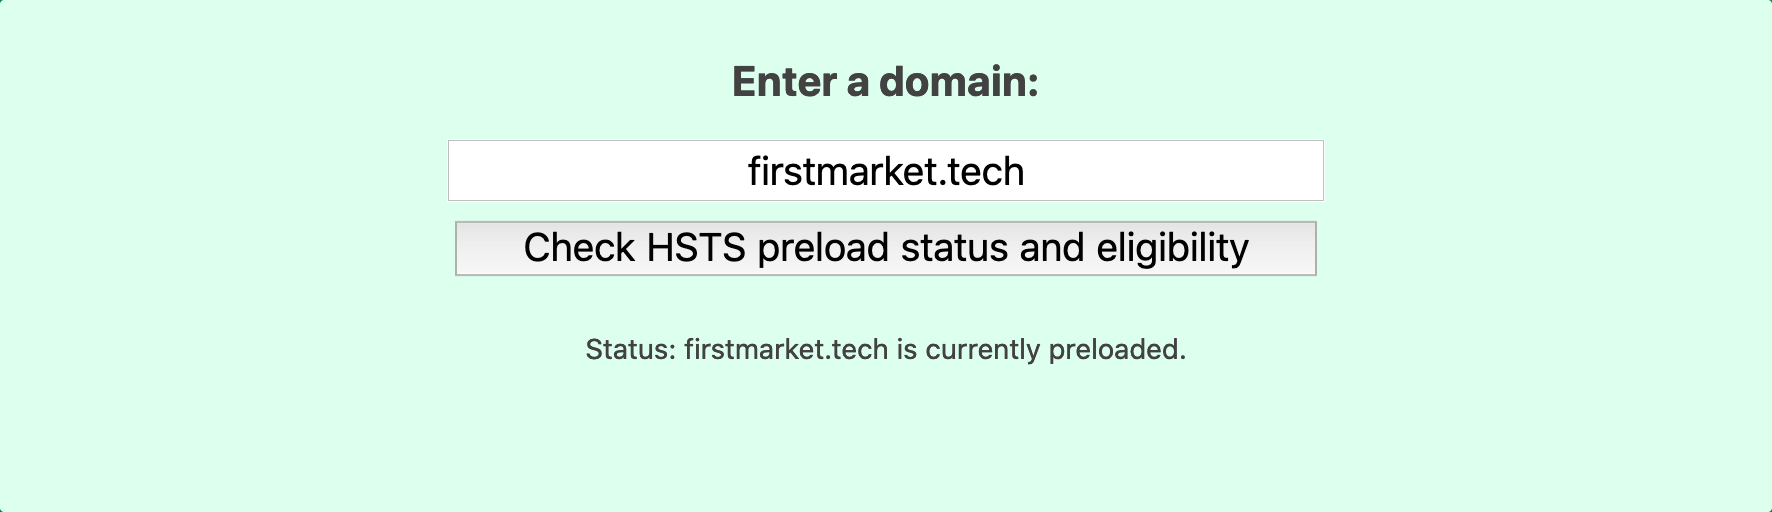
\includegraphics[width=\textwidth,keepaspectratio]{hsts_preload}
		\caption{Confirmación de la inclusión en la lista de dominios web \emph{HSTS preload}}
		\label{fig:hsts_preload}
	\end{figure}
	
	Otra forma es incluyendo el encabezado \emph{Strict-Transport-Security} en las respuestas HTTP. En las líneas de la 46 a la 51 del listado \ref{list:springsec_config} se muestra la configuración realizada en Spring Security para incluir la cabecera mostrada en el listado \ref{list:hsts} en las respuestas HTTP.
	\\
	
	\begin{lstlisting}[caption=Cabecera de declaración \emph{HSTS host}, label=list:hsts]
	 Strict-Transport-Security: max-age=31536000 ; includeSubDomains ; preload
	\end{lstlisting}
	
	\paragraph{X-Frame-Options}
	Con el objetivo de prevenir los ataques conocidos como \href{https://en.wikipedia.org/wiki/Clickjacking}{\emph{clickjacking}}, Spring Security inhabilita el renderizado de vistas que contengan etiquetas HTML5 \emph{iframe}. Esto se consigue enviando a los navegadores el encabezado que se muestra en el listado \ref{list:iframe}.
	\\
	
	\begin{lstlisting}[caption=Cabecera que inhibe el uso de las etiquetas \emph{iframe}, label=list:iframe]
	 X-Frame-Options: DENY
	\end{lstlisting}
	
	\paragraph{X-XSS-Protection}
	Muchos navegadores implementan filtros anti-\href{https://owasp.org/www-community/attacks/xss/}{XSS}. Aún no representando una solución infalible al problema, ayudan mucho a su mitigación. Normalmente estos filtros están habilitados por defecto, siendo posible configurar qué hacer en caso de un positivo (por ejemplo, intentar enmendar el contenido detectado).
	
	Spring Security, por defecto, a través del encabezado que se muestra en el listado \ref{list:filtro_xss}, activa explícitamente el filtro del navegador y lo configura para que ante un positivo bloquee el contenido.
	\\
	
	\begin{lstlisting}[caption=Cabecera que activa y configura el filtro anti-XSS del navegador, label=list:filtro_xss]
	X-XSS-Protection: 1; mode=block
	\end{lstlisting}
	
	\paragraph{Content Security Policy}
	La \href{https://developer.mozilla.org/en-US/docs/Web/HTTP/CSP}{\emph{Content Security Policy}} (CSP) es un mecanismo de protección frente a vulnerabilidades de inyección de contenido, como por ejemplo el comentado \href{https://owasp.org/www-community/attacks/xss/}{\emph{cross-site scripting}}. A través de esta funcionalidad se puede declarar y, en última instancia, informar al navegador acerca de cuáles son las fuentes autorizadas desde las cuales descargar los recursos que las vistas de la aplicación web necesita.
	
	Esta política de permisos, no trivial, depende de las necesidades de cada sitio web, y es por ello que Spring Security no la configura por defecto. Así, en el listado \ref{list:springsec_config}, entre las líneas X y Y, se declara la CSP de la aplicación web desarrollada. Como se aprecia, se especifican diversas fuentes para distintos tipos de contenido. Es importante resaltar que tanto con los \emph{scripts} como con las hojas de estilo debe evitarse su uso en modo \emph{inline}, esto es, embebido en el propio HTML, usando en su lugar ficheros \emph{.js} y \emph{.css}.
	
	\paragraph{Referrer  Policy}
	Uno de los muchos encabezados que se incluyen en una petición HTTP es el \href{https://developer.mozilla.org/en-US/docs/Web/HTTP/Headers/Referer}{\emph{Referer}}, que contiene la dirección de la página web anterior desde la cual se realizó la navegación a la página actual. Por otro lado, el encabezado \href{https://developer.mozilla.org/en-US/docs/Web/HTTP/Headers/Referrer-Policy}{\emph{Referrer-Policy}} controla qué restricciones aplicar a la información suministrada en el encabezado \emph{Referer}.
	
	Es importante establecer un criterio apropiado ya que, por ejemplo, si no se especifica política alguna que restrinja la información contenida en el encabezado \emph{Referer}, este podría contener el token de seguridad que FirstMarket adjunta en el link que envía a los usuarios para verificar la dirección de correo electrónico. En general, la información sensible que puedan contener las URL quedaría expuesta en el encabezado \emph{Referer}.
	
	Spring Security permite de una manera sencilla configurar la política deseada, que en el caso de FirstMarket ha sido \textbf{\emph{strict-origin}}, como se aprecia en las líneas 76 y 79 del listado \ref{list:springsec_config}. Esta política establece que sólo se envía información en el encabezado \emph{Referer} si el destinatario usa HTTPS. Esta es la parte \emph{strict} de \emph{strict-origin}. La parte \emph{origin} significa que sólo se envía el origen de la dirección. Por ejemplo, de \emph{www.firstmarket.tech/login?error=true} sólo sería enviado \emph{www.firstmarket.tech}.
	
	\paragraph{Subresource Integrity}
	Por último, y aunque no se trate de una funcionalidad ofrecida por Spring Security, es necesario comentar que la aplicación web desarrollada hace uso del mecanismo conocido como \href{https://www.w3.org/TR/SRI/}{\emph{Subresource Integrity}}. 
	
	Se trata de una protección destinada a mitigar la vulnerabilidad que entraña depender de librerías (u otros recursos) de terceros. Por ejemplo, si la librería de jQuery se viera comprometida, automáticamente lo estaría también todas las aplicaciones que hacen uso de la misma. Así, para prevenir que se pueda inyectar código en algún recurso del que se dependa, y este sea propagado sin detección, esta técnica introduce metadatos de integridad en la declaración de la fuente. Estos metadatos están ligados al contenido original, así que si este se viese modificado el navegador lo detectaría y lo bloquearía.
	
	Los metadatos son un código \emph{hash} criptográfico obtenido a partir del contenido original de la dependencia (como ya se ha comentado, Git emplea la misma estrategia para detectar cambios en los ficheros que gestiona). Estos códigos se pueden obtener de muchas maneras. La presente aplicación web los ha obtenido de \href{https://www.srihash.org/}{srihash.org}. En el listado \ref{list:sri} se muestra un ejemplo de esta técnica, en el que FirstMarket declara la dependencia con la librería JavaScript jQuery.
	\\
	
	\begin{lstlisting}[caption=Subresource Integrity, label=list:sri]
	<script src="https://ajax.googleapis.com/ajax/libs/jquery/3.5.1/jquery.min.js"
		integrity="sha384-ZvpUoO/+PpLXR1lu4jmpXWu80pZlYUAfxl5NsBMWOEPSjUn/6Z/hRTt8+pR6L4N2"
		crossorigin="anonymous">
	</script>
	\end{lstlisting}
	
	\paragraph{Resultados}
	Para finalizar con este apartado, a continuación, en las figuras \ref{fig:moz_scan_summary} y \ref{fig:moz_scan_results}, se muestran los resultados obtenidos por \href{https://firstmarket.tech}{www.firstmarket.tech} en el test \href{https://observatory.mozilla.org/analyze/www.firstmarket.tech}{\emph{Mozilla Observatory}}, al aplicar las políticas de seguridad descritas en los párrafos anteriores.
	
	\begin{figure}[hbt!]
		\centering
		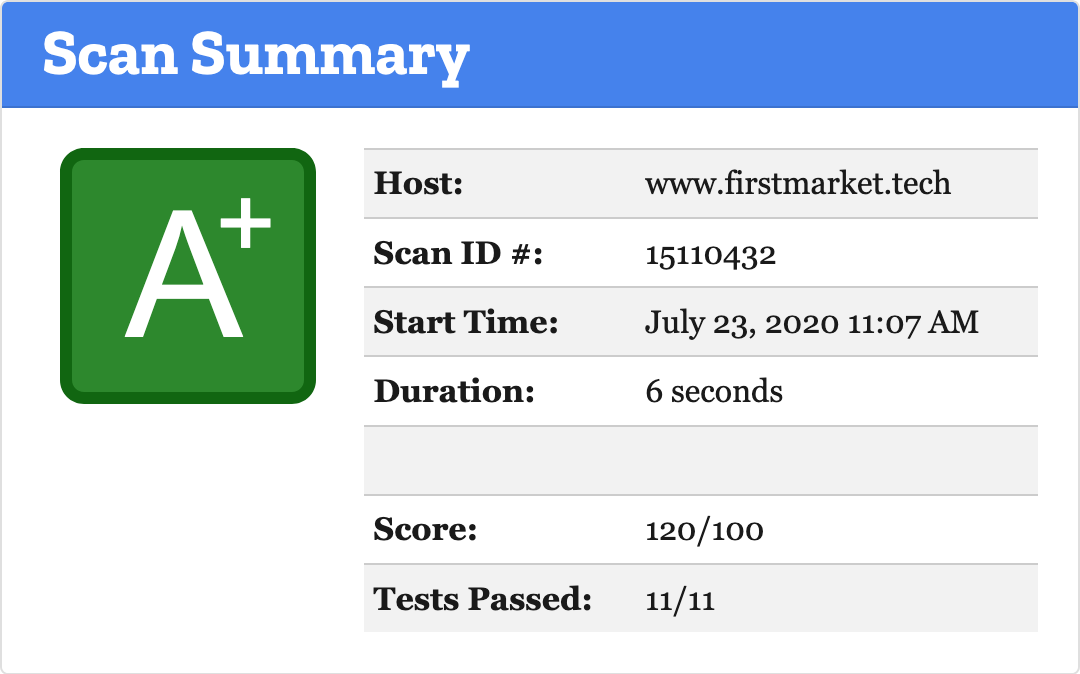
\includegraphics[width=0.6\textwidth,keepaspectratio]{moz_scan_summary}
		\caption{Resumen del test \emph{Mozilla Observatory}}
		\label{fig:moz_scan_summary}
	\end{figure}

	\begin{figure}[hbt!]
		\centering
		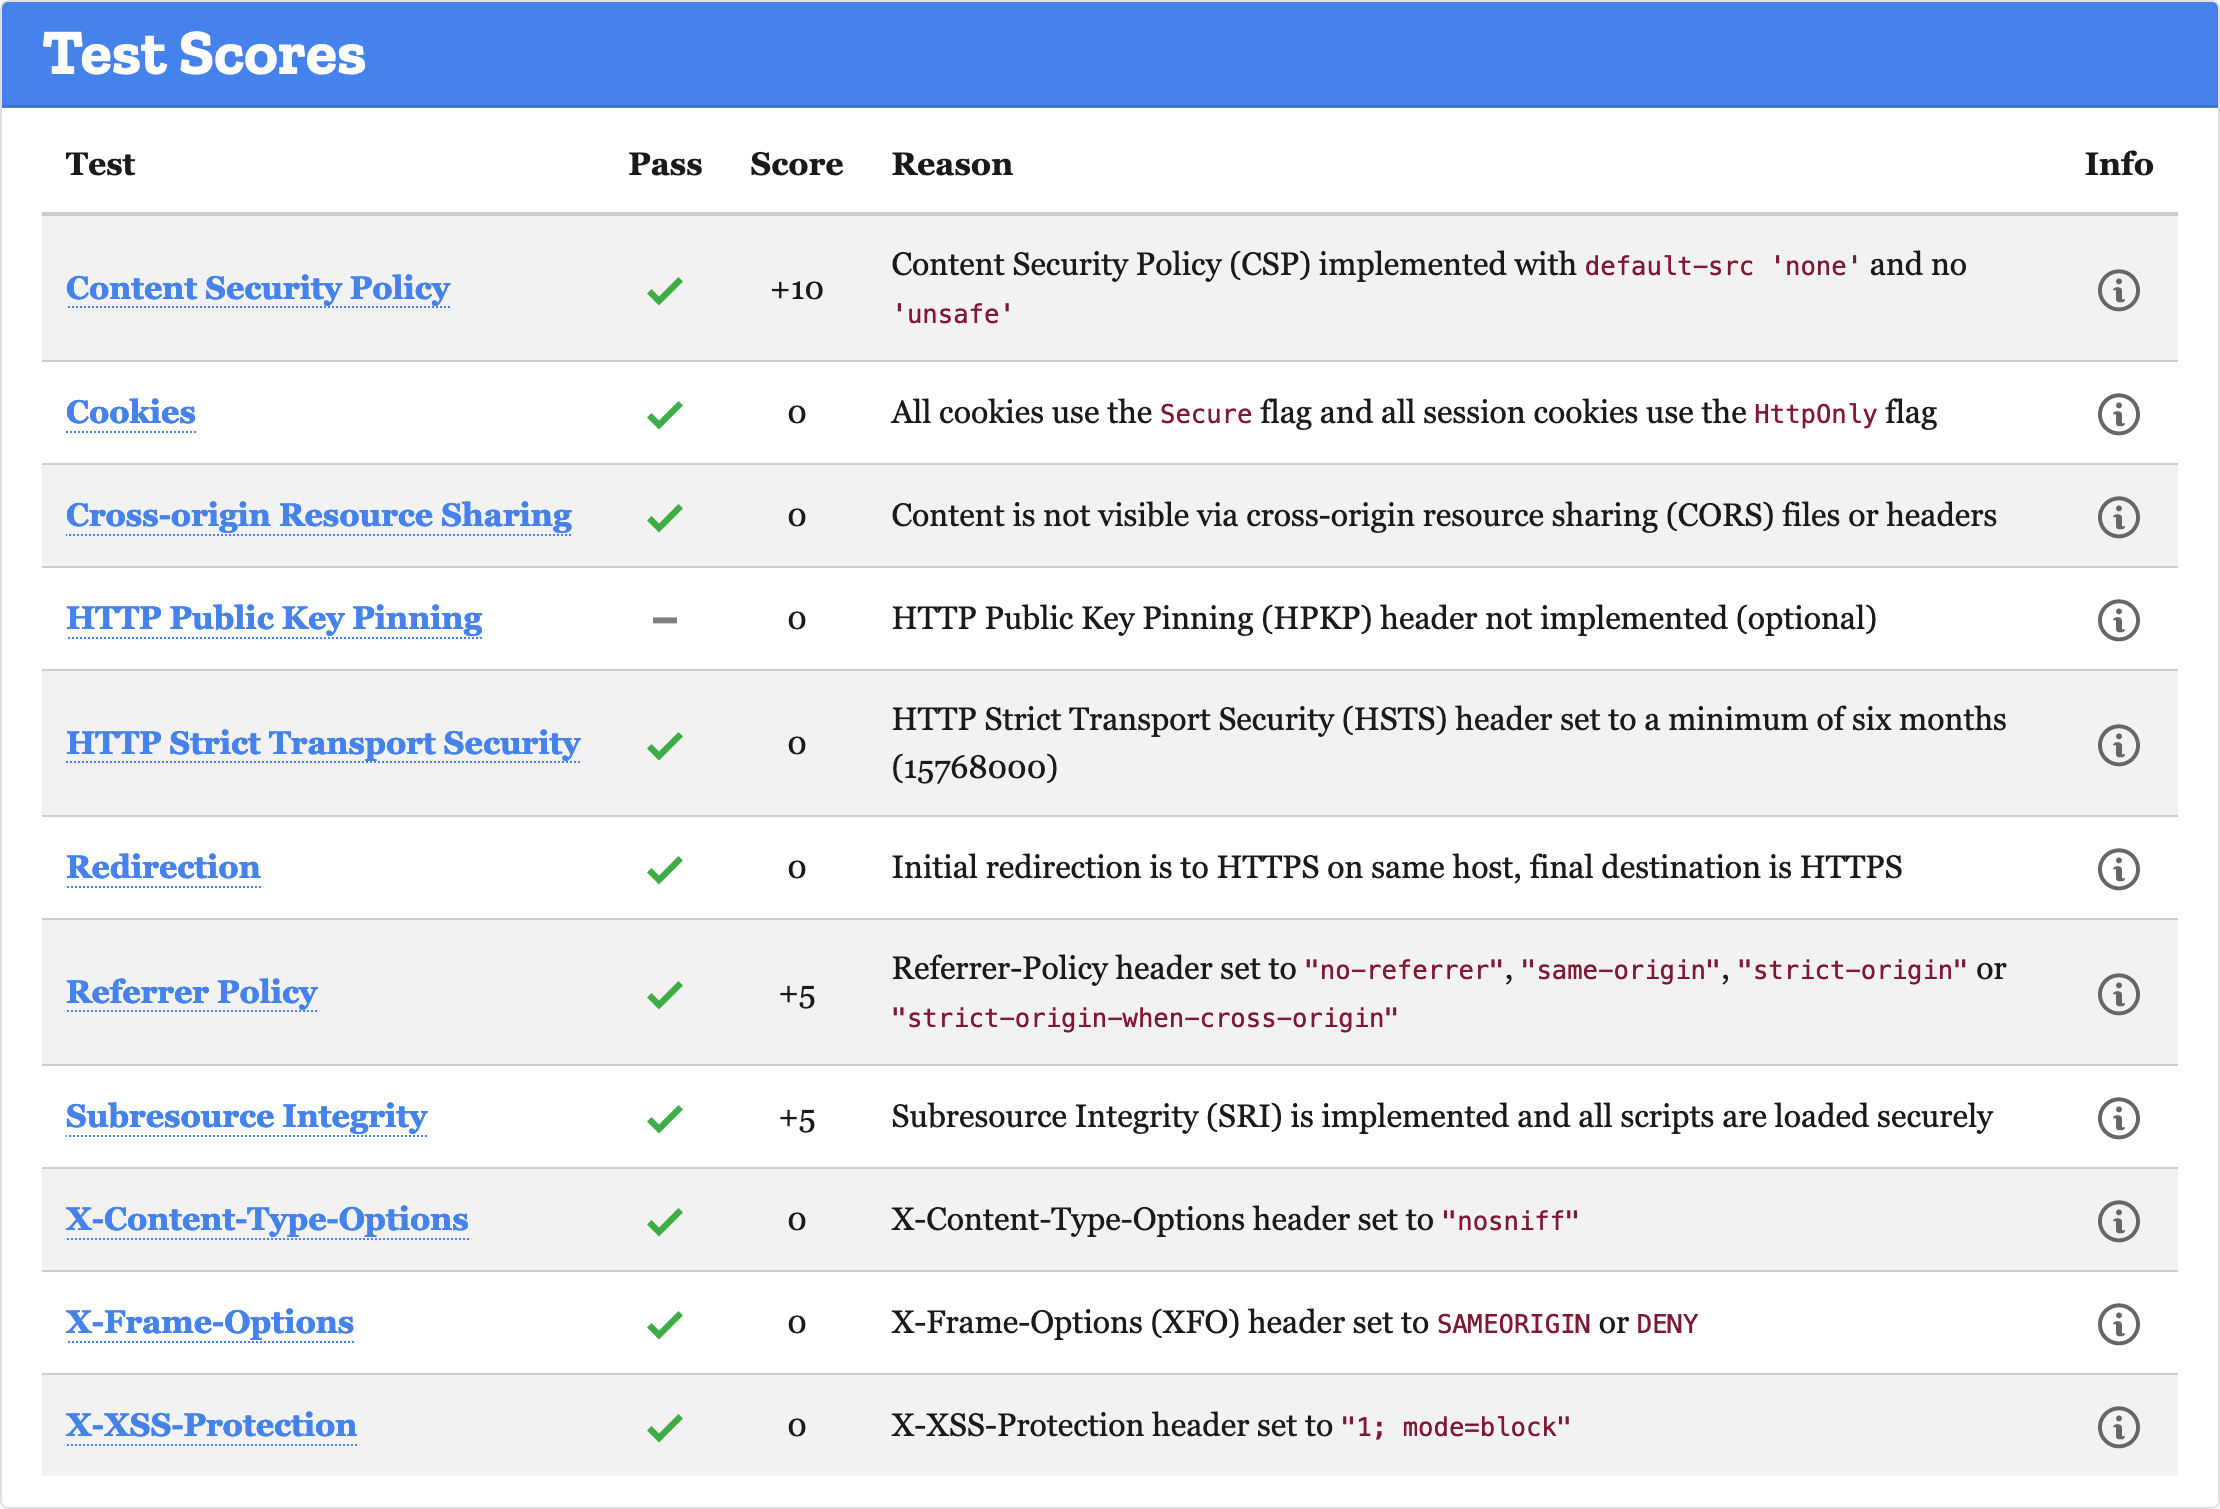
\includegraphics[width=\textwidth,keepaspectratio]{moz_scan_results}
		\caption{Resultados del test \emph{Mozilla Observatory}}
		\label{fig:moz_scan_results}
	\end{figure}
	
	\section{Validación de Entradas}
	Por validación se entiende las comprobaciones que la aplicación web hace sobre los datos que le son proporcionados externamente. El caso más común es cuando un usuario envía un formulario cumplimentado a la aplicación web, y esta, antes de procesar la información, comprueba que se cumplen ciertas reglas. Por ejemplo, puede requerirse que el campo de email sea efectivamente una dirección de correo válida, o que la fecha de nacimiento sea una fecha pasada válida (nadie puede nacer el 30 de febrero, por ejemplo). Esto se hace para garantizar la consistencia de los datos en la base de datos y, quizás más importante, para evitar ataques de inyección de contenido.
	
	Esta comprobación se puede hacer tanto en cliente como en servidor. Desde el punto de vista de la seguridad, realizar la comprobación en servidor es \textbf{obligatorio}, ya que las comprobaciones en cliente son muy fácilmente circunvaladas. Por otro lado, desde el punto de vista de la experiencia de usuario es muy recomendable implementarla también en cliente, ya que permite al usuario tener un \emph{feedback} mucho más rápido que si debiese esperar a que el servidor responda. En definitiva, la mejor práctica es implementar la validación tanto en \emph{backend} como en \emph{frontend}, y así se ha implementado en la aplicación web desarrollada. Resaltar, además, que los componentes de validación en \emph{backend} están en el paquete \emph{util.validation}.
	
	Mucha es la información que FirstMarket debe validar, pero a grandes rasgos se puede dividir en numérica y textual. El primer grupo presenta poca dificultad, se trata de comprobar rangos de valores principalmente. Para el segundo grupo las expresiones regulares son el arma perfecta. En el archivo de configuración \emph{application.yml} se detallan las expresiones regulares y los rangos numéricos utilizados. A modo de ejemplo, la propiedad definida en este archivo de configuración que especifica la expresión regular contra la que validar las contraseñas se muestra en el listado \ref{list:regex_pw}.
	\\
	
	\begin{lstlisting}[caption=Expresión regular para las contraseñas,label=list:regex_pw]
	fm:
		validation:
			regex:
				password: ^(?=.*\d)(?=.*[a-z])(?=.*[A-Z]).{8,16}$
	\end{lstlisting}
	
	Así, esta expresión regular es utilizada por la aplicación web para comprobar, tanto en \emph{frontend} como en \emph{backend}, que cuando un usuario proporciona una nueva contraseña esta tenga una longitud de entre 8 y 16 caractéres e incluya al menos una minúscula, una mayúscula y un dígito.
	
	Existe un campo que destaca por su manera de ser validado. Se trata del ISBN (International Standard Book Number) de los libros. Este campo necesita validación en dos vertientes. La primera se realiza utilizando las ya mencionadas expresiones regulares, pero, para validar si se trata de un ISBN válido, aún hay que calcular el dígito de control y comprobar que coincida con el último dígito del código. Los ISBN tuvieron 10 dígitos hasta diciembre de 2006, pero desde entonces tienen siempre 13 (ambas versiones con diferentes algoritmos de cálculo del dígito de control). Así pues, la validación implementada en FirstMarket da soporte a ambos formatos de ISBN.
	
	\section{Análisis de Vulnerabilidades} \label{sec:vulnerabilities}
	Como se comentó en la sección \ref{sec:addons}, la seguridad de la aplicación web ha sido testada con la ayuda de \href{https://probely.com/}{Probely} y \href{https://snyk.io/}{Snyk}. La primera herramienta detectó 5 vulnerabilidades, mientras que la segunda 13. Del total, 14 responden a vulnerabilidades conocidas en librerías utilizadas por la aplicación web, por lo que su resolución se basa en actualizar las versiones de dichas dependencias. A continuación se pasa a comentar los problemas encontrados, haciendo especial énfasis en las 4 vulnerabilidades propias de la aplicación web desarrollada: 
	
	\begin{itemize}
		\item[-] \textbf{\emph{Reflected cross-site scripting}}. Esta vulnerabilidad, considerada de \textbf{alto riesgo}, fue encontrada durante el test OWASP top 10 realizado con Probely.
		
		Este riesgo se encuentra bastante extendido por Internet y ocurre cuando el servidor de la aplicación toma un input del cliente y lo devuelve nuevamente sin validar o codificar adecuadamente para ser mostrado por pantalla. El adjetivo \emph{reflected} proviene del código malicioso que se envía al servidor y se refleja en el navegador de la víctima en el código fuente de la página.
		
		En el caso concreto de la presente aplicación, esta vulnerabilidad se encontró en la vista de las categorías, \emph{categories.html}. En esta vista, como se explica en la sección \ref{sec:hierarchy}, el código HTML necesario para mostrar la estructura de categorías anidadas se genera dinámicamente con \emph{categoriesBuilder.js}. Para que este \emph{script} pueda realizar su función, el servidor incrusta dentro de \emph{categories.html} la información de las categorías en formato JSON.
		\\
		
		\begin{lstlisting}[caption=Extracto de categories.html con la vulnerabilidad encontrada,label=list:rcss_template]
		...
		<!-- categories dynamically generated -->
		<i id="catHolder" th:attr="jsonStringCategories=${jsonStringCategories}"></i>
		<!-- insecure: reflected XSS
		<script th:utext="'let jsonStringCats = \'' + ${jsonStringCategories} + '\';'"></script>
		-->
		<script th:src="@{/js/categoriesBuilder.js}"></script>
		...
		\end{lstlisting}
		
		Como se aprecia en la línea 5 del listado \ref{list:rcss_template}, la manera vulnerable de hacer disponible la información de categorías a \emph{categoriesBuilder.js} es haciendo uso de la directiva de Thymeleaf \textbf{\emph{th:utext}} en la declaración de la variable JavaScript \emph{jsonStringCats}, donde la \emph{u} significa \emph{unscaped}. Esta manera de renderizar la información del servidor es el origen del problema, ya que los caracteres especiales que puedan contener los nombres de las categorías no son apropiadamente codificados.
		
		Una manera segura, que resuelve el problema, es la implementada en la línea 3 del mismo listado \ref{list:rcss_template}, donde se utiliza la directiva de Thymeleaf \emph{th:attr} para incrustar la estructura JSON como un atributo HTML. Esta directiva sí codifica adecuadamente los caracteres especiales, mitigando el riesgo de insertar código malicioso en el nombre de las categorías y que sea servido y expuesto a los clientes.
		
		\begin{figure}[hbt!]
			\centering
			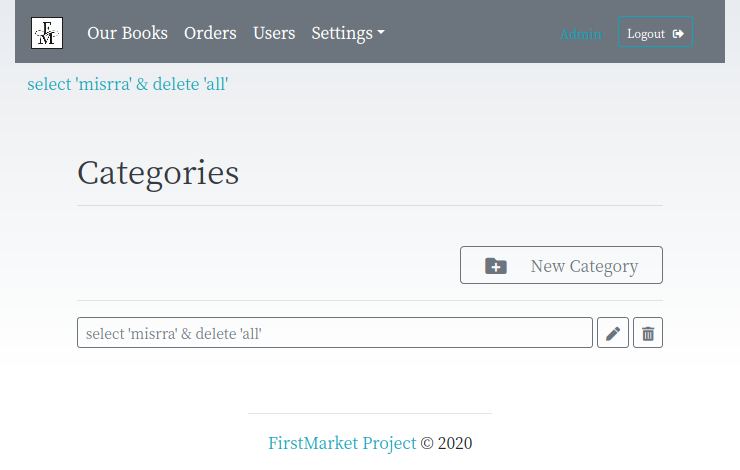
\includegraphics[width=\textwidth,keepaspectratio]{cat_rcss}
			\caption{Categoría con caracteres especiales en su nombre}
			\label{fig:cat_rcss}
		\end{figure}
		
		En la figura \ref{fig:cat_rcss} se muestra un nombre de categoría con caracteres especiales, exponiéndose en el listado \ref{list:rcss_html} un extracto de su código fuente, generado con ambos métodos: el seguro en la línea 3 y el inseguro, sin codificar los caracteres, en la línea 5.
		\\
		
		\begin{lstlisting}[caption=Extracto del HTML generado a partir del template categories.html,label=list:rcss_html]
		...
		<!-- categories dynamically generated -->
		<i id="catHolder" jsonStringCategories="{ &quot;name&quot;:&quot;firstmarket&quot;, &quot;id&quot;:6, &quot;children&quot;:[{ &quot;name&quot;:&quot;select &#39;misrra&#39; &amp; delete &#39;all&#39;&quot;, &quot;id&quot;:68, &quot;children&quot;:[]}]}"></i>
		<!-- insecure: reflected XSS 
		<script>let jsonStringCats = '{ "name":"firstmarket", "id":6, "children":[{ "name":"select 'misrra' & delete 'all'", "id":68, "children":[]}]}';</script>
		-->
		<script src="/js/categoriesBuilder.js"></script>
		...
		\end{lstlisting}
		
		\item[-] \textbf{\emph{Potential DoS on TLS Client Renegotiation}}. Esta vulnerabilidad (\href{https://nvd.nist.gov/vuln/detail/CVE-2011-1473}{CVE-2011-1473}) está basada en la asimetría de trabajo que tiene lugar cuando el cliente inicia una renegociación de los parámetros criptográficos de una conexión TLS con el servidor, soportando este la mayor carga de trabajo. Así, un cliente malicioso podría iniciar una conexión TLS y seguidamente requerir el procedimiento de renegociación repetidas veces, en busca de colmar los recursos del servidor.
		
		La renegociación para acordar nuevos parámetros de cifrado se desarrolla dentro de una única conexión TCP. Esto es clave, ya que otros ataques DoS relacionados con TLS se basan en inundar al servidor con nuevas conexiones TCP, contra lo cual muchos cortafuegos implementan algún tipo de control del ritmo de peticiones de nuevas conexiones TCP. Pero esta vulnerabilidad explota que la renegociación tiene lugar dentro de una única conexión TCP, evitando así este tipo de controles.
		
		Para controlar esta amenaza en la aplicación web desarrollada sería necesario implementar una restricción sobre el ratio de peticiones de renegociación iniciadas por el cliente, o simplemente deshabilitar esta capacidad. Se ha optado por la segunda opción, dada la sencillez de su implementación y el bajo o nulo impacto en la experiencia de usuario. Así, para deshabilitar esta opción, Java 8 introdujo una nueva variable de la JVM, de forma que únicamente es necesario invocar la aplicación con la opción detallada en el listado \ref{list:tls_renegotiation}.
		\\
		
		\begin{lstlisting}[caption=Deshabilitado del inicio por parte del cliente de la renegociación TLS,label=list:tls_renegotiation]
		-Djdk.tls.rejectClientInitiatedRenegotiation=true
		\end{lstlisting}
		
		\item[-] \textbf{\emph{Outdated TLS protocol version 1.0 supported}}. Como se explica en la sección \ref{sec:https}, Heroku ofrece conexiones seguras con TLS, por defecto, a través de su funcionalidad \href{https://devcenter.heroku.com/articles/automated-certificate-management}{\emph{Automated Certificate Management}}. La vulnerabilidad descrita en este apartado se produce por el hecho de que ACM no fuerza el uso de TLS v1.2+, es decir, no deshabilita el uso de versiones obsoletas de TLS.
		
		Tal como se explica en su \href{https://devcenter.heroku.com/articles/understanding-ssl-on-heroku#when-to-use-the-ssl-endpoint}{documentación}, para deshabilitar el soporte a las versiones inseguras, TLS v1.0 y TLS v1.1, sería necesario sustituir ACM por \href{https://devcenter.heroku.com/articles/ssl-endpoint}{SSL Endpoint}, el cual es un servicio con un coste de 20 dólares mensuales.
		
		Teniendo en cuenta el coste indicado, y la reciente (8 Jul 2020) notificación recibida desde Heroku, mostrada a seguir, se ha optado por continuar usando ACM:
		
		\begin{displayquote}
			Dear Heroku Customer,
			\\
			
			At Salesforce, our top priority is providing you with a trusted Heroku platform, and today we begin our migration off of older, less secure TLS versions with a plan to completely block TLS v1.0/v1.1 next year after July 31, 2021. [...]
			\\
			
			Heroku currently supports TLS v1.0/v1.1, as well as the latest, more secure TLS v1.2+ protocol on all apps. [...]
			\\
			
			Today, Heroku begins implementing these recommendations to transition all apps to TLS v1.2+, so that we can End of Life TLS v1.0/v1.1 next year. [...]
			\\
			
			Beginning on June 1, 2021, we will begin migration all apps to the new cipher suites and block TLS v1.0/v1.1 completing this migration by July 31, 2021. 
			\\
			
			After July 31, 2021, clients that access Heroku apps using TLS v1.0/v1.0 will be blocked. [...]
			\\
			
			Sincerely, Heroku.
		\end{displayquote}
		
		\item[-] \textbf{\emph{Referrer policy not defined}}. La vulnerabilidad comentada en este punto se debe a que no se había especificado qué política de \emph{Referer} emplear, con el consecuente riesgo de enviar información sensible en dicho encabezado. Como se explica en la sección \ref{sec:springsec}, el riesgo queda mitigado al especificar la política \emph{strict-origin} con Spring Security.
		
		\item[-] \textbf{\emph{Vulnerabilidades en librerías de terceros}}. Las restantes 14 vulnerabilidades se han solucionado por medio de actualizaciones. Por la propia naturaleza de la herramienta, todas los problemas detectados por Snyk entran dentro de este epígrafe, mostrándose en la figura \ref{fig:snyk} dos de las vulnerabilidades más graves que ha detectado. Las actualizaciones realizadas han sido las siguientes:
		
		\begin{itemize}
			\item[1.] org.springframework.boot:spring-boot $\rightarrow$ 2.3.1.RELEASE
			\item[2.] org.springframework:spring-web $\rightarrow$ 5.2.4.RELEASE
			\item[3.] org.springframework:spring-webmvc $\rightarrow$ 5.2.4.RELEASE
			\item[4.] org.hibernate:hibernate-core $\rightarrow$ 5.4.18.Final
			\item[5.] org.springframework.security:spring-security-core $\rightarrow$ 5.3.2.RELEASE
			\item[6.] org.apache.tomcat.embed:tomcat-embed-core $\rightarrow$ 9.0.37
			\item[7.] org.webjars:jquery $\rightarrow$ 3.5.1
		\end{itemize}
		
		\begin{figure}[hbt!]
			\centering
			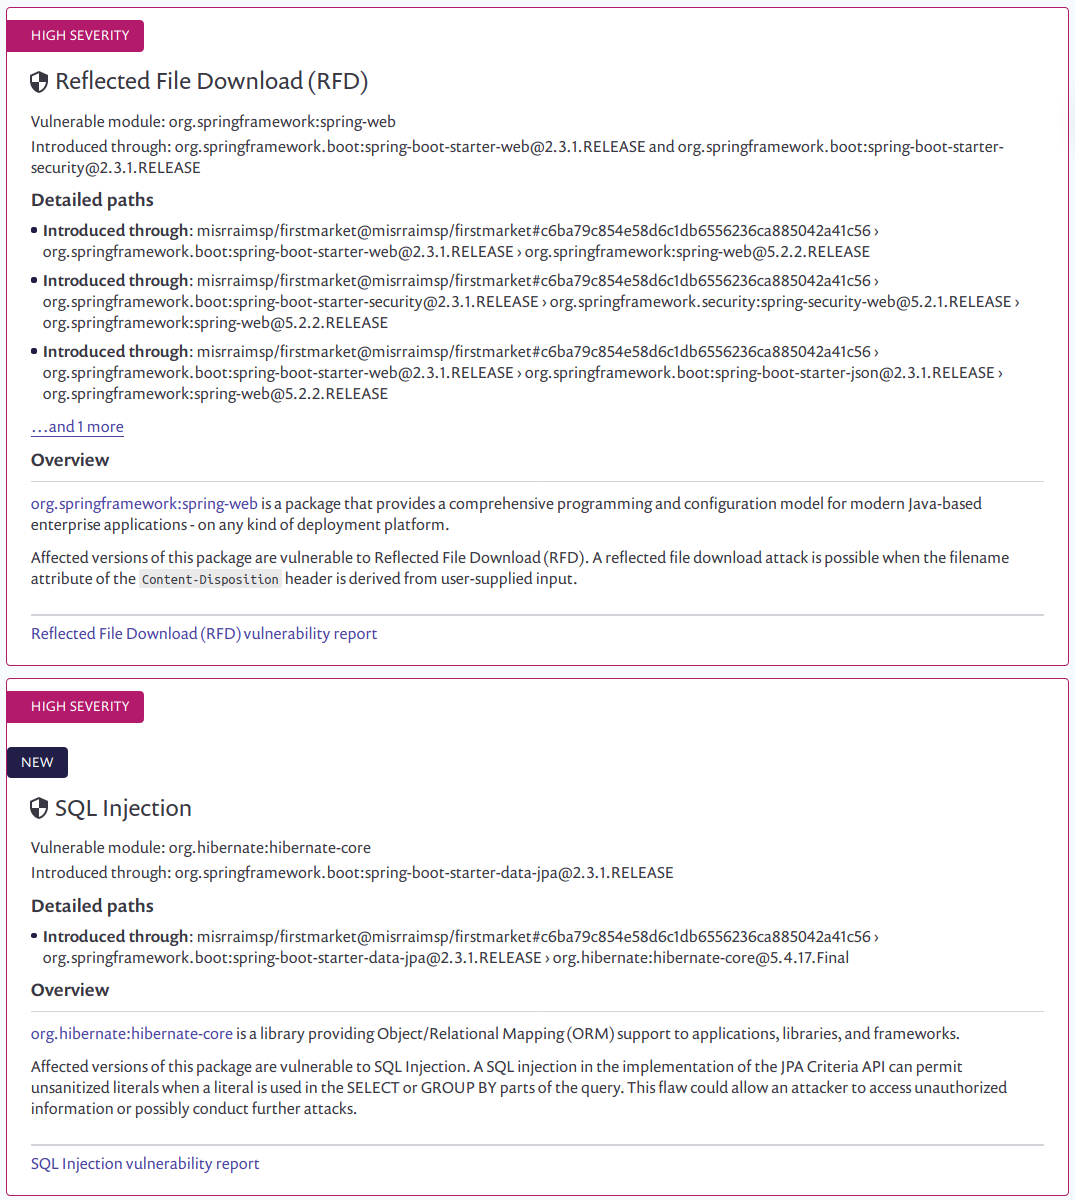
\includegraphics[width=\textwidth,keepaspectratio]{snyk}
			\caption{Ejemplo de vulnerabilidades encontradas por Snyk}
			\label{fig:snyk}
		\end{figure}
		
		Un aspecto que debe resaltarse es que las actualizaciones de la 2 a la 6, incluidas ellas, han tenido que establecerse sobrescribiendo la configuración que por defecto ofrece Spring Boot a través del fichero \emph{spring-boot-starter-parent}, del cual hereda el \emph{pom.xml} de la aplicación web desarrollada. Esto es importante porque se está saliendo del terreno seguro que esta configuración por defecto suministra, en el sentido de que desde Spring se ha testado que las versiones establecidas por defecto funcionan sin problemas de compatibilidades entre sí.
		
	\end{itemize}